%%%%%%%%%%%%%%%%%%%%%%%%%%%%%%%%%%%%%%%%%%%%%%%%%%%%%%%%%%%%%%%%%%%%%%
% LaTeX Template: Beamer arrows
%
% Source: http://www.texample.net/
% Feel free to distribute this template, but please keep the
% referal to TeXample.net.
% Date: Nov 2006
% 
%%%%%%%%%%%%%%%%%%%%%%%%%%%%%%%%%%%%%%%%%%%%%%%%%%%%%%%%%%%%%%%%%%%%%%


\documentclass{beamer} %
\usetheme{CambridgeUS}
\usepackage[utf8]{inputenc}
\usefonttheme{professionalfonts}
\usepackage{times}
\usepackage{tikz}
\usepackage{amsmath}
\usepackage{graphicx}
\usepackage{url}
\usepackage{array} % needed for \arraybackslash
\usepackage{adjustbox} % for \adjincludegraphics
\usepackage{subcaption}
\usepackage{verbatim}
\usetikzlibrary{arrows,shapes}
\usepackage[absolute,overlay]{textpos}
\usepackage[cache=false]{minted}
\usepackage{pdfcomment}
\captionsetup{compatibility=false}
\usepackage{url}

\newcommand{\pdfnote}[1]{\marginnote{\pdfcomment[icon=note]{#1}}}

%alex special colors
\usepackage{color}

\definecolor{alexred}{RGB}{239,138,98}
\definecolor{alexgreen}{RGB}{145,207,96}
\definecolor{alexblue}{RGB}{103,169,207}


% gets rid of bottom navigation bars
%\setbeamertemplate{footline}[page number]{}

% gets rid of navigation symbols
\setbeamertemplate{navigation symbols}{}

% add figures numbering
\setbeamertemplate{caption}[numbered]


%source information

\newcommand{\source}[1]{\begin{textblock*}{3.9cm}(8.8cm,8.8cm)
		\begin{beamercolorbox}[ht=0.3cm,right]{framesource}
			\usebeamerfont{framesource}\usebeamercolor[fg]{framesource} \tiny Source: {#1}
		\end{beamercolorbox}
\end{textblock*}}

\begin{document}

\author{Pascal Escher\textsuperscript{1}, Philipp Thiel\textsuperscript{2}}
\title[Git]{Version Control with Git}
\institute[ABI]{1 Applied Bioinformatics, University of Tübingen\\2 Interfaculty Institute for Biomedical Informatics, University of Tübingen\\}
\date{April 08\textsuperscript{th}, 2021}
\setbeamertemplate{footline}[page number]{}

\maketitle

\begin{frame}
\frametitle{Most important help}
\begin{center}

	
\includegraphics[scale=0.18]{assets/google_classic.jpg}

	... btw ...  do you know this awesome service? \\
	... \url{https://lmgtfy.com}

\end{center}
\end{frame}

\begin{frame}
\frametitle{FYI}

The intention of this course is to bring the people with least IT skills to a point where
they can start their masters courses in bioinformatics. If you're a fast one and manage to
solve todays issues in a short time please be patient! Here are some interesting things you
can read in the meantime:

\begin{itemize}
    \setlength\itemsep{1em}
	\item About Git: \\ \url{http://tom.preston-werner.com/2009/05/19/the-git-parable.html}
	\item Microsoft and GitHub: \\ \url{https://medium.com/@ow/microsoft-acquiring-github-is-a-good-thing-heres-why-6a6a57eb83ac}
    \item Dilbert: \url{http://dilbert.com}
    \item PhdComics: \url{http://www.phdComics.com}
\end{itemize}
\end{frame}

%Basic concepts of git: Why do we need it? Why do we want it? 
\begin{frame}[t]
\frametitle{Git: Motivation}
\begin{itemize}
    \setlength\itemsep{1em}
	\item Git is one software for VERSION CONTROL \newline
    \item It's not the only one
    
	\begin{itemize}
    	\setlength\itemsep{0.4em}
		\item Subversion (SVN)
        \item Mercurial
        \item Perforce 
        \item Deprecated: Concurrent Versions System (CVS)
        \item \href{https://en.wikipedia.org/wiki/List_of_version_control_software}{https://en.wikipedia.org/wiki/List\_of\_version\_control\_software} 
	\end{itemize}
    
    \item However, maybe it's nowadays the most popular one ...
    
\end{itemize}
\end{frame}

\begin{frame}[t]
\frametitle{Git: Inventor}
\begin{center}
	
	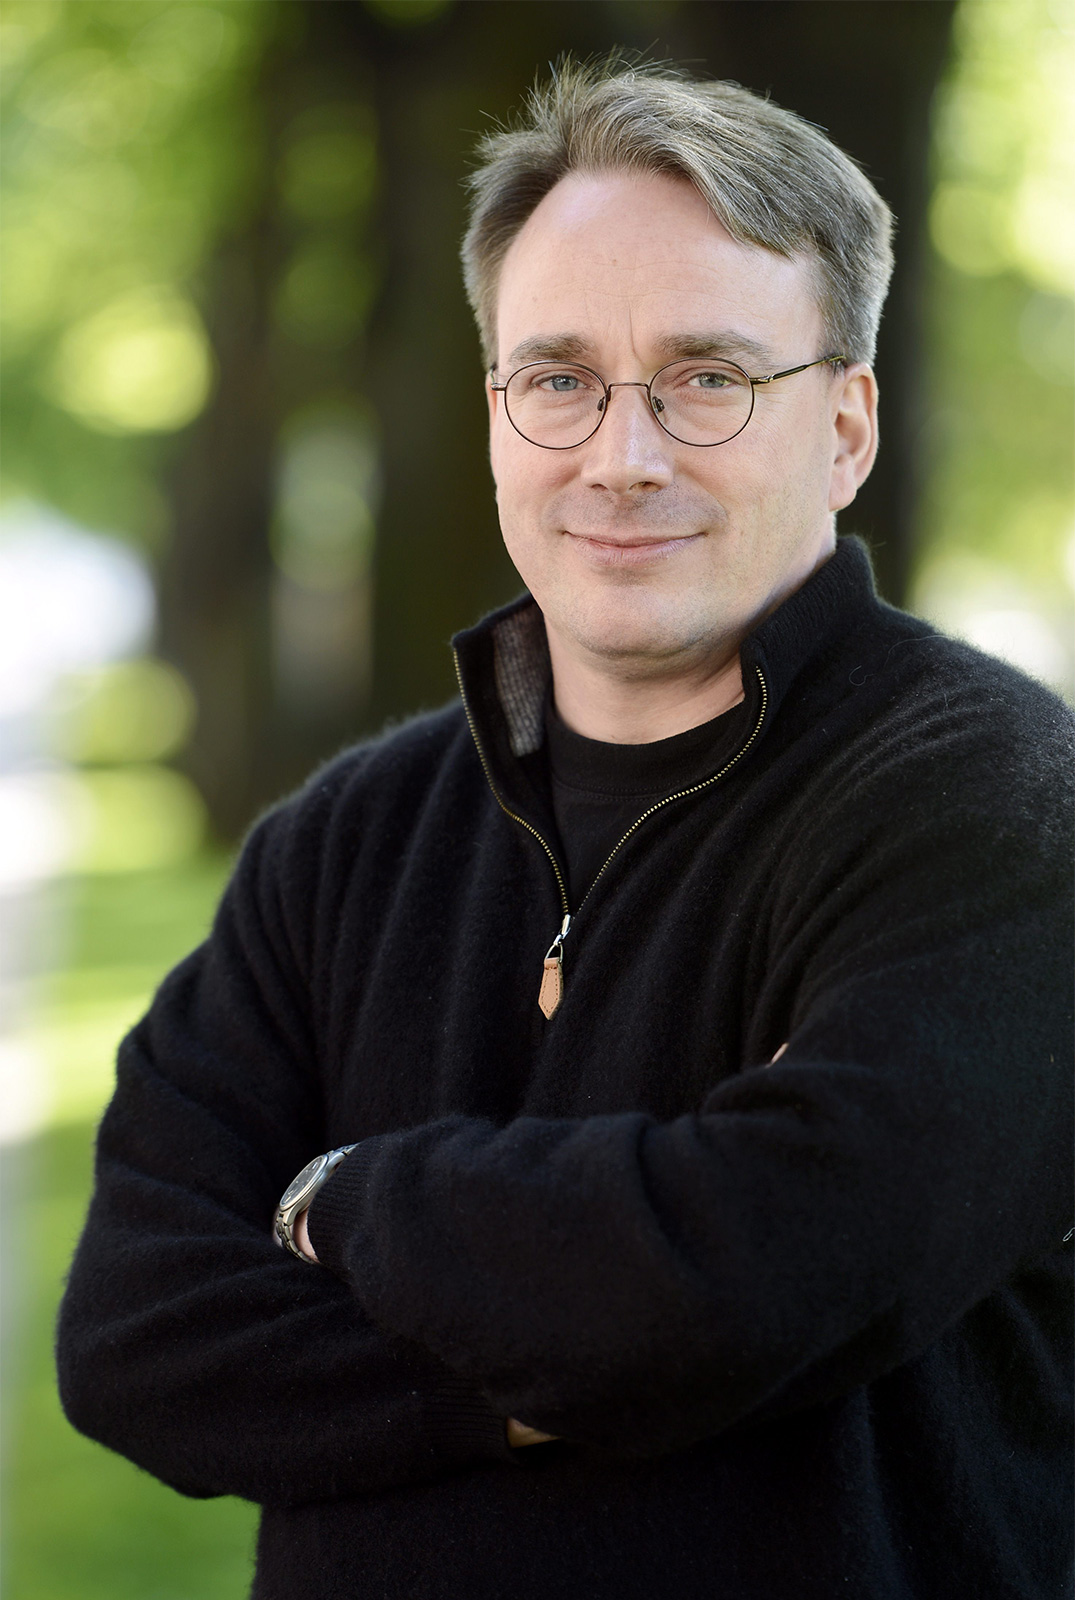
\includegraphics[scale=0.10]{assets/Linus-Torvalds-2012.jpg}
	
	One of the founder of Linux and Git: Linus Torvalds\\
	Source: \url{https://cdn.britannica.com/}
	
\end{center}
\end{frame}

\begin{frame}[t]
\frametitle{Git: Github}
	\begin{center}
		
		\includegraphics[scale=0.75]{assets/Microsoftbiggestdeals.png}
		
		Microsoft bought GitHub in 2018 for 7,5 billion \$\\
		Source: \url{https://www.geekwire.com/2018/heres-microsofts-github-acquisition-ranks-among-tech-giants-largest-deals/}
		
	\end{center}
\end{frame}

\begin{frame}[t]
\frametitle{Git: Important Resources}
\begin{itemize}
    \setlength\itemsep{1em}
	\item The docu and installer \newline \url{https://git-scm.com} \newline
    \item A nice tutorial \newline \url{https://try.github.io/levels/1/challenges/1} \newline
    \item Maybe to be read first \newline \url{http://tom.preston-werner.com/2009/05/19/the-git-parable.html} \newline
\end{itemize}
\end{frame}

\begin{frame}[t]
\frametitle{Git \& Software Projects}
\begin{figure}
    \begin{center}
    	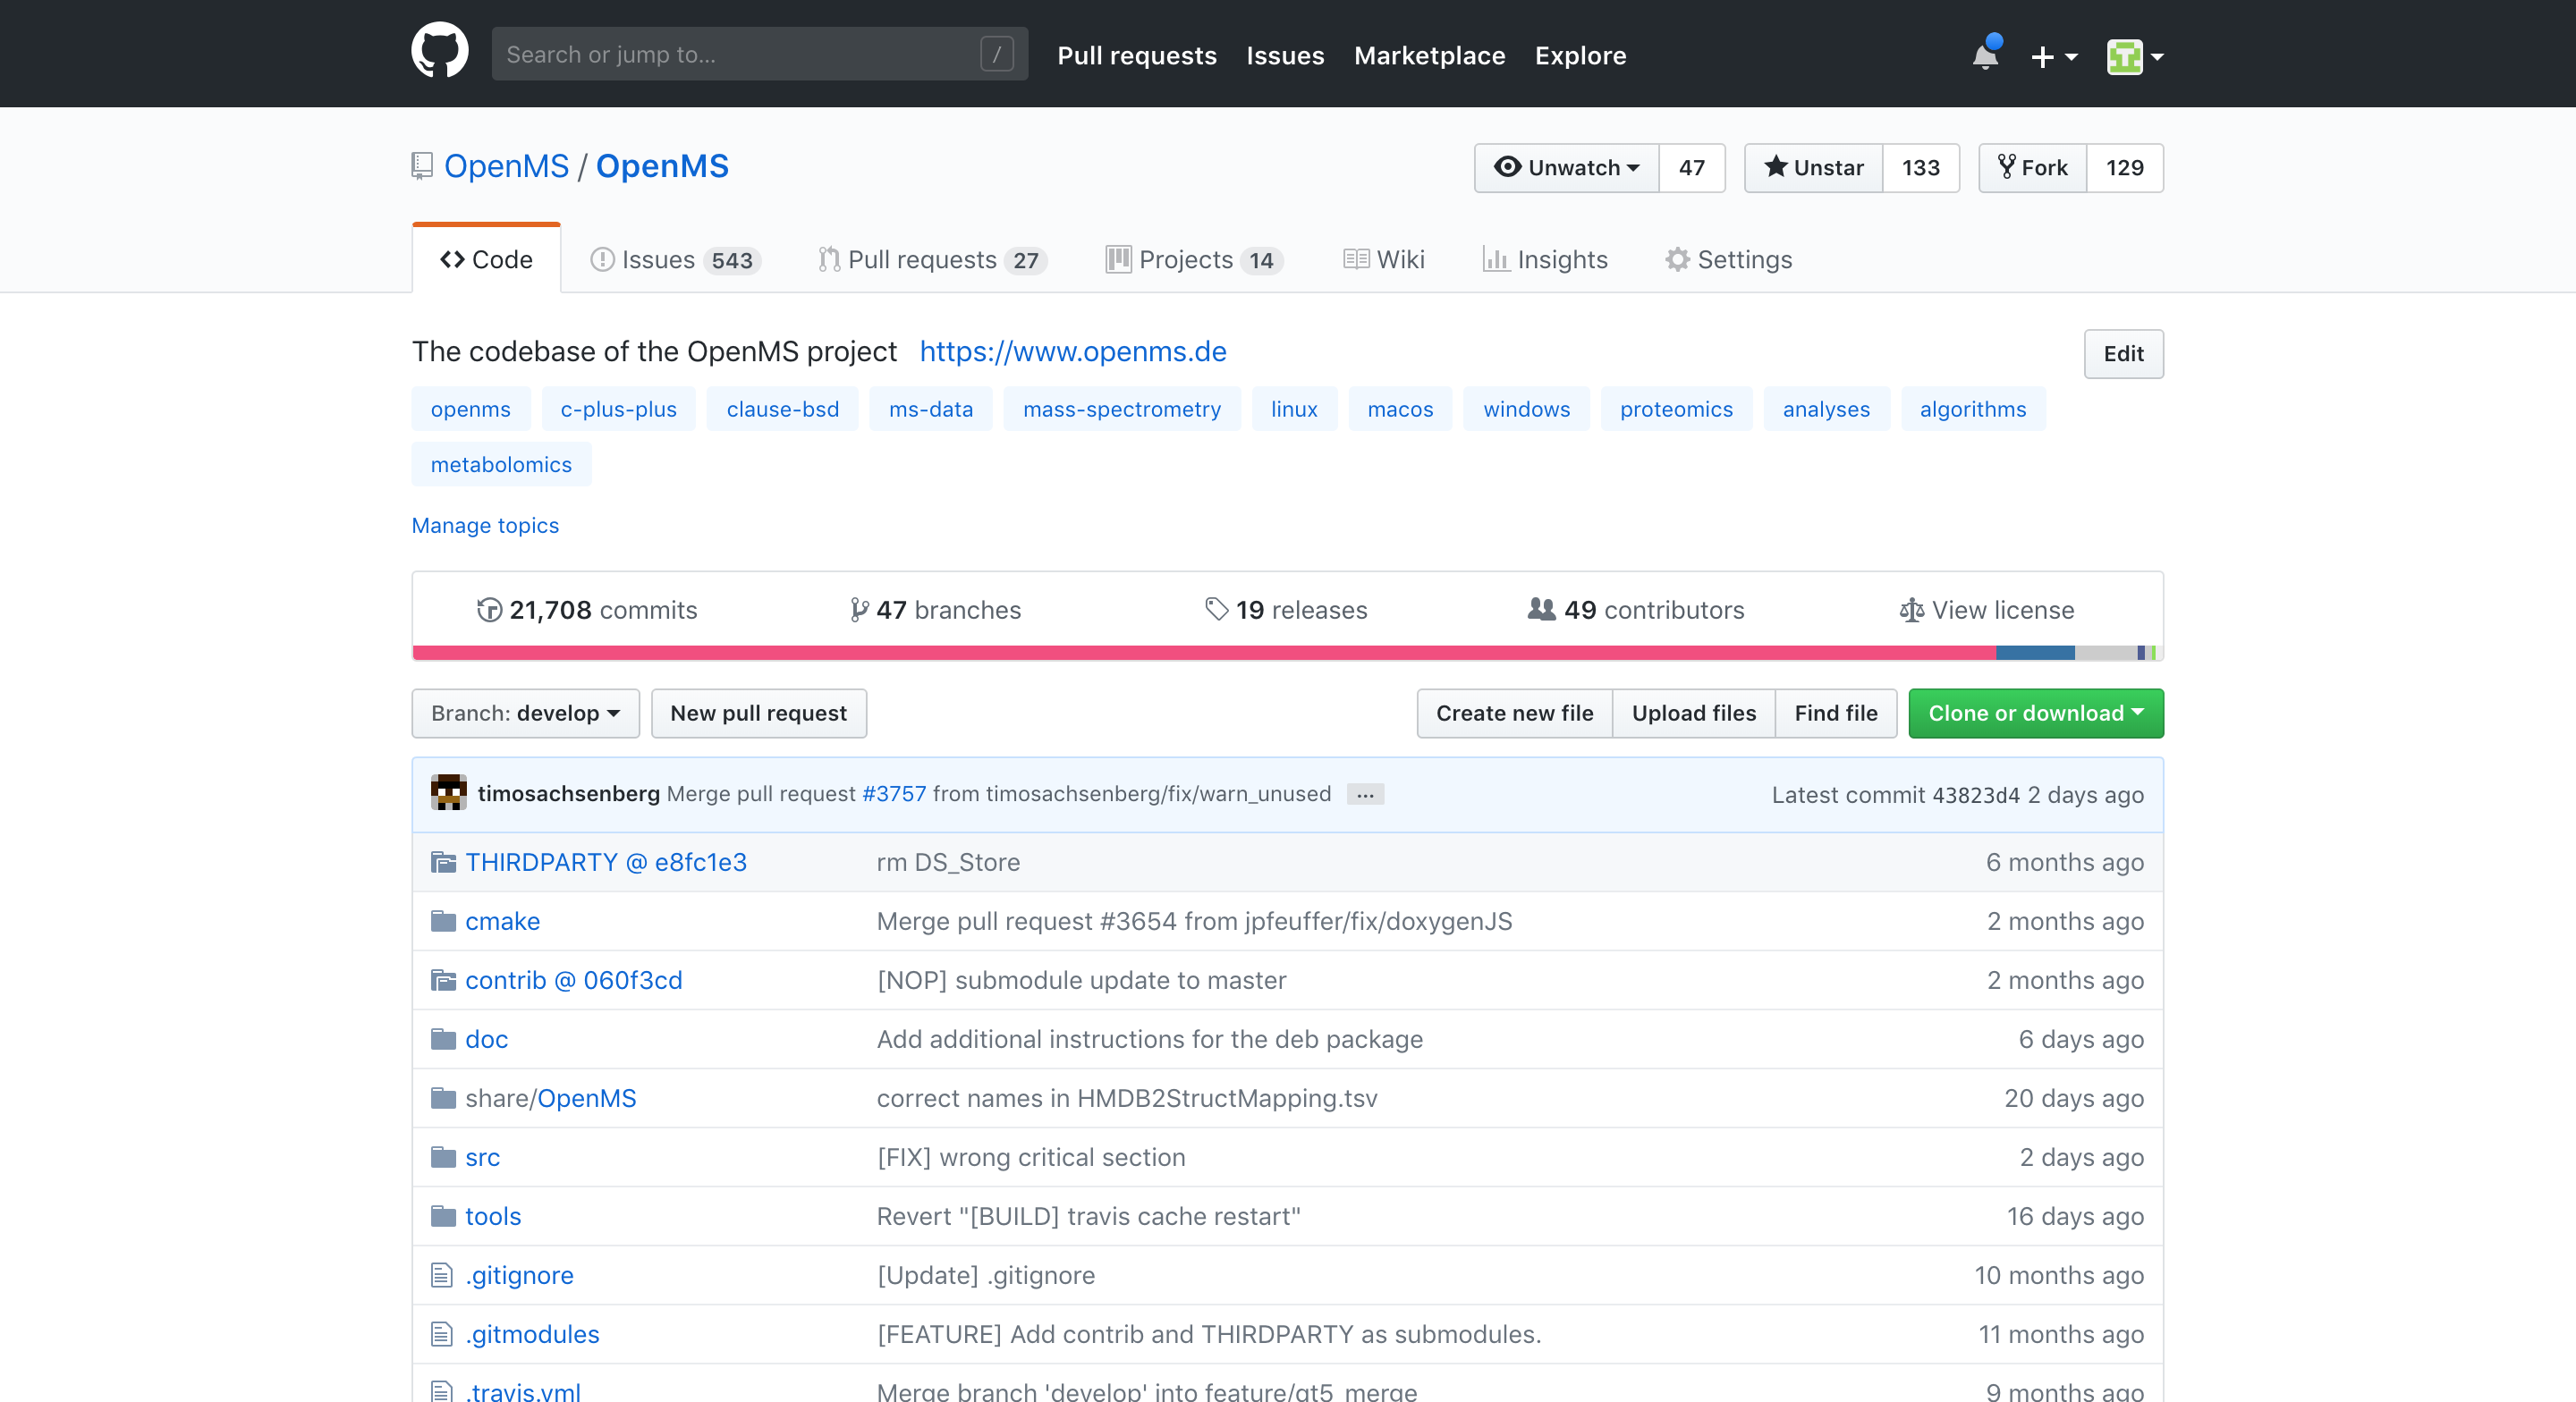
\includegraphics[width=0.7\textwidth]{assets/OpenMS.png}
    \end{center}
\end{figure} 
\begin{itemize}
    \setlength\itemsep{1em}
	\item Version Control is indispensable for bigger software projects with lots of developers, 
	e.g. https://github.com/OpenMS/OpenMS
    \item Useful for smaller projects/application/scripts as well! \newline
\end{itemize}
\end{frame}

\begin{frame}[t]
\frametitle{Git \& Software Projects}
You can depict a local repository by three trees. The first one is the working directory, which holds the files. The second is an index which is used as staging area. The last one is head, which points to your last commit. Git saves the changes you make and stores it in the index/head based on adding and commit the changes.
\begin{figure}
    \begin{center}
    	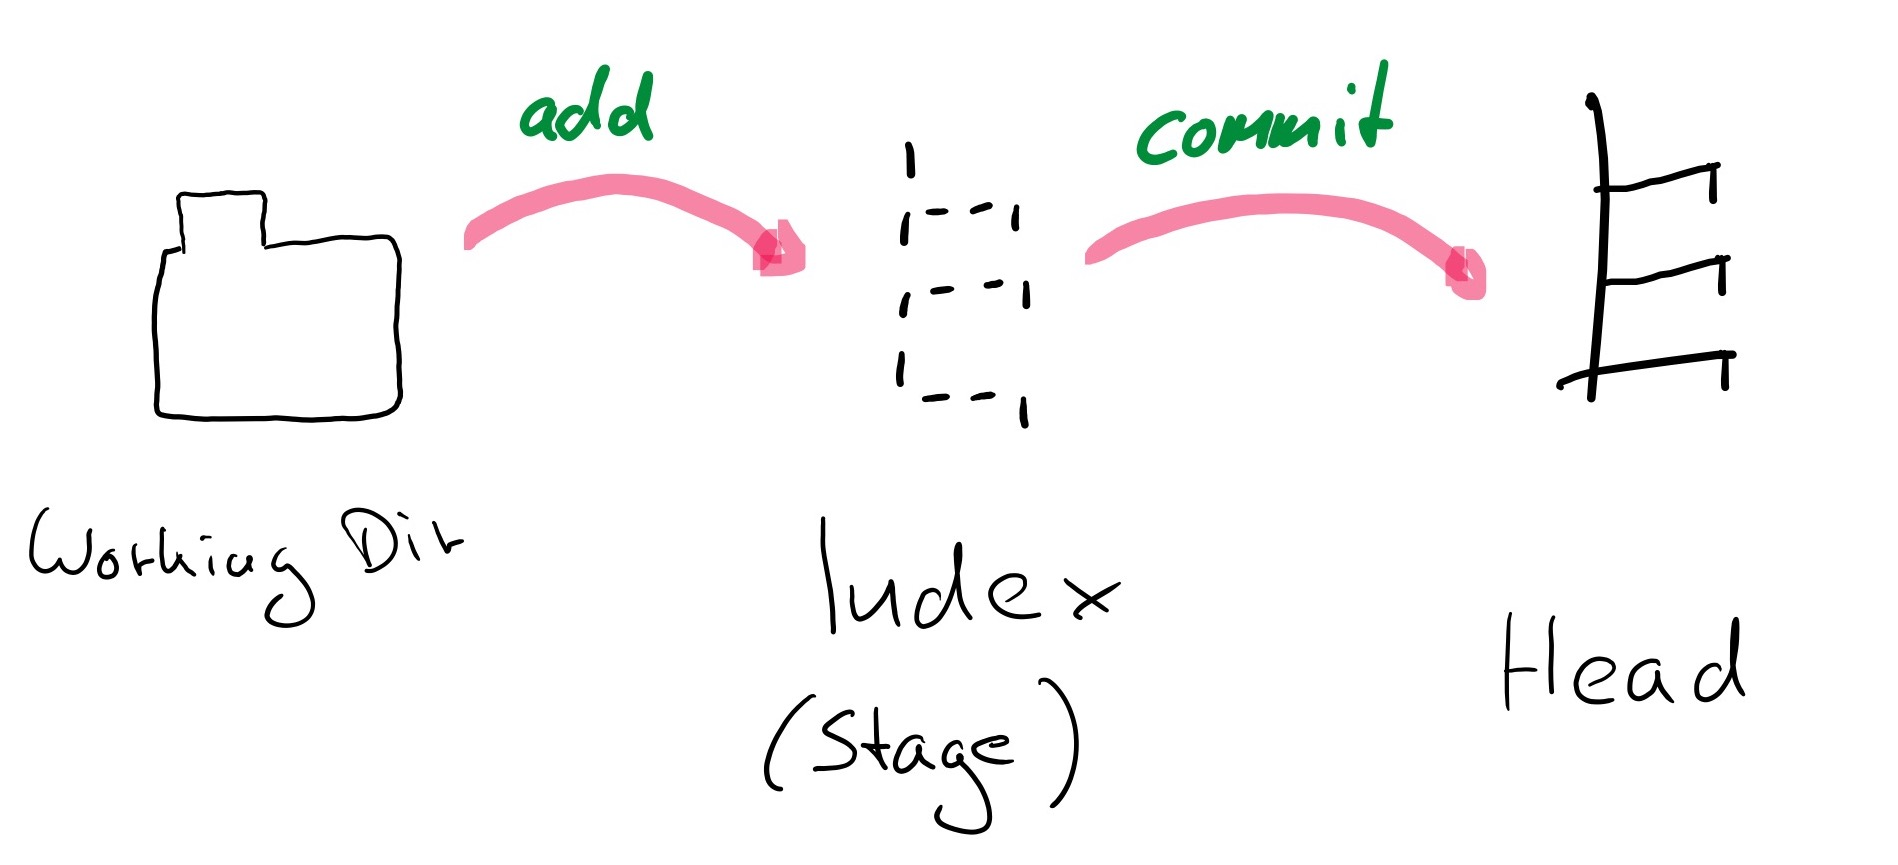
\includegraphics[width=\textwidth]{assets/git.jpg}
    \end{center}
\end{figure}
\end{frame}

\begin{frame}[t]
\frametitle{Git \& Software Projects}

\begin{figure}
    \begin{center}
    	\includegraphics[width=\textwidth]{oa_git_1.pdf}
    \end{center}
\end{figure}
\end{frame}

\begin{frame}[t]
\frametitle{Git \& Software Projects}
\begin{figure}
    \begin{center}
    	\includegraphics[width=\textwidth]{oa_git_2.pdf}
    \end{center}
\end{figure}
\end{frame}

\begin{frame}[t]
\frametitle{Git \& Software Projects}

\begin{figure}
    \begin{center}
    	\includegraphics[width=0.7\textwidth]{oa_git_3.pdf}
    \end{center}
\end{figure}
\end{frame}

\begin{frame}[t]
\frametitle{Git \& Software Projects}
Prerequisites:
\begin{itemize}
\item Create an account for Github (https://github.com)
\item Install git \url{https://git-scm.com/book/en/v2/Getting-Started-Installing-Git}
\item Note: You can use the VirtualBox Image (Linux course) - if you like. 
\item Create a new empty directory and change into it.
\item Note: If you run into a problem when using git, please read the info/error message in the terminal carefully - usually it is self explaining. If you get stuck - give google a chance. If nothing helps, don't hesitate to ask! 
\end{itemize}
\end{frame}

\begin{frame}[t, fragile]
\frametitle{How to proceed}
In the first set, we have a look at basic git commands. \\
\\
We create a local repository and play around with it. \\
\\
The following slides are separated into commands and Task sets. \\
\\
Please have a peak at the Task Set first! \\
\\
Then check the following "important commands", play around with them and
try to solve the given tasks. 
\end{frame}

\begin{frame}[t, fragile]
\frametitle{Git: Important Commands}

\begin{minted}[mathescape, numbersep=5pt, frame=lines]{latex} 
 $ git init
\end{minted}

\begin{itemize}
    \setlength\itemsep{1em}
	\item Create a new empty repository
    \item Play around in the directory, e.g. create a new folder
    \item Check the git status
\end{itemize}

\begin{minted}[mathescape, numbersep=5pt, frame=lines]{latex} 
 $ git status
\end{minted}
\end{frame}

\begin{frame}[t, fragile]
\frametitle{Git: Important Commands}

\begin{itemize}
    \setlength\itemsep{1em}
    \item Create a new text file and write something into it ...
    \item ... and check the status again
\end{itemize}

\begin{minted}[mathescape, numbersep=5pt, frame=lines]{latex} 
 $ git status
\end{minted}

\end{frame}


\begin{frame}[t, fragile]
\frametitle{Git: Important Commands}

\begin{minted}[mathescape, numbersep=5pt, frame=lines]{latex} 
 $ git add
\end{minted}

\begin{itemize}
    \setlength\itemsep{1em}
	\item Purpose: Prepare changes for integration into your repo
\end{itemize}


\begin{minted}[mathescape, numbersep=5pt, frame=lines]{latex} 
 $ git add -A
\end{minted}

\begin{itemize}
    \setlength\itemsep{1em}
	\item Add everything that is not ignored
\end{itemize}


\end{frame}

\begin{frame}[t, fragile]
\frametitle{Git: Important Commands}

\begin{minted}[mathescape, numbersep=5pt, frame=lines]{latex} 
 $ git commit
\end{minted}

\begin{itemize}
	\setlength\itemsep{1em}
	\item Purpose: Integrate added changes into your repo
\end{itemize}

\begin{minted}[mathescape, numbersep=5pt, frame=lines]{latex} 
 $ git commit -m "important-commit-message"
\end{minted}

\begin{itemize}
	\setlength\itemsep{1em}
	\item Commit - adding a commit message directly
\end{itemize}

\begin{minted}[mathescape, numbersep=5pt, frame=lines]{latex} 
 $ git commit --amend
\end{minted}

\begin{itemize}
	\setlength\itemsep{1em}
	\item Correct last commit wrt files and message
\end{itemize}
\end{frame}

\begin{frame}[t, fragile]
\frametitle{Git: Important Commands}

\begin{minted}[mathescape, numbersep=5pt, frame=lines]{latex} 
 $ git reset HEAD <file> $
\end{minted}

\begin{itemize}
    \setlength\itemsep{1em}
	\item Unstage a file (Undo adding)
\end{itemize}
\end{frame}

\begin{frame}[t, fragile]
\frametitle{Git: Important Commands}

\begin{minted}[mathescape, numbersep=5pt, frame=lines]{latex} 
 $ git log
\end{minted}

\begin{itemize}
	\setlength\itemsep{1em}
	\item Purpose: Check commit history
\end{itemize}
\end{frame}



\begin{frame}[t, fragile]
\frametitle{Git: Task Set 1}

\begin{enumerate}
	\item Download the following archive:
    \url{https://www.dropbox.com/s/y2bwsfvv2ctn6a9/awesome_project.zip?dl=0}
    \item Extract \verb|awesome_project.zip| somewhere in your file system
    \item Initialize \verb|awesome_project/| to a Git repository
    \item Add source files, but not the config and .class files
    \item Make a commit
    \item Try to find out how to ignore config and .class files (So they won't be added 
    with git -A)
    \item If you are fast: Reset your repo to previous commit (Try to find out how to use git reset)
\end{enumerate}

\end{frame}

\begin{frame}[t, fragile]
\frametitle{Git: Some Preliminary Work}

\begin{itemize}
    \setlength\itemsep{1em}
	\item Purpose: Get a copy of our work project in your GitHub account (peek at Task2)
    \item To do this we fork the repository (repo) of interest
    \item Go the the online repository and use the fork button. Now you have a fork and can edit it as you like! \begin{figure}
    \begin{center}
    	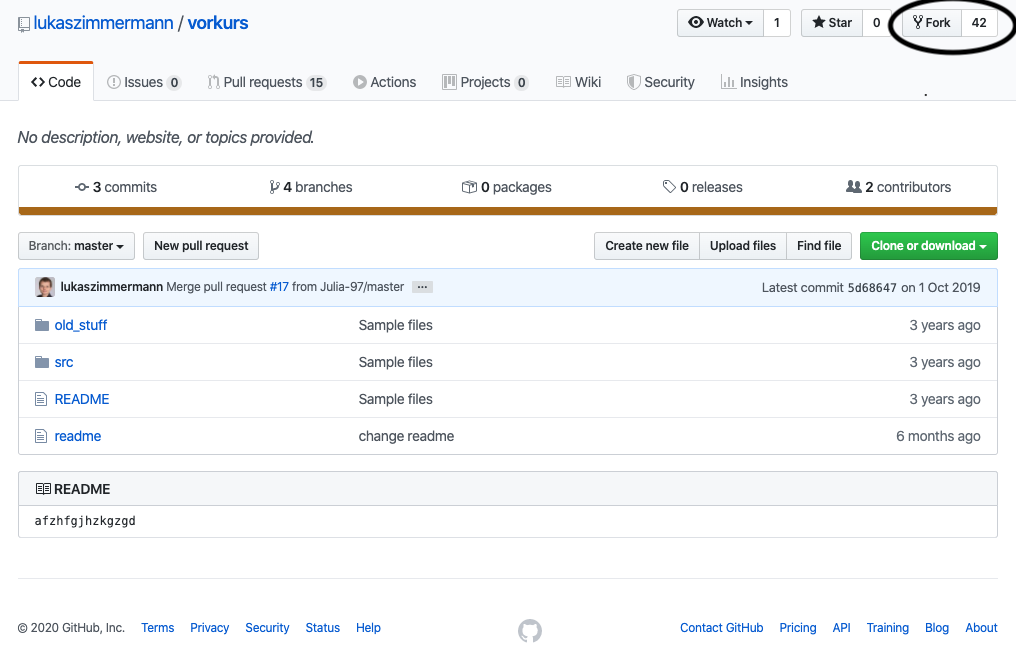
\includegraphics[width=0.7\textwidth]{assets/fork.png}
    \end{center}
\end{figure}   
\end{itemize}
\end{frame}

\begin{frame}[t, fragile]
\frametitle{Git: Important Commands}

\begin{minted}[mathescape, numbersep=5pt, frame=lines]{latex} 
 $ git clone
\end{minted}

\begin{itemize}
    \setlength\itemsep{1em}
	\item Purpose: Get a local copy of your remote repo (project)
    \item How does this work?
    \item Let's get help
\end{itemize}

\begin{minted}[mathescape, numbersep=5pt, frame=lines]{latex} 
 $ git clone -h
\end{minted}

\end{frame}

\begin{frame}[t, fragile]
\frametitle{Git: Important Commands}

\begin{minted}[mathescape, numbersep=5pt, frame=lines]{latex} 
 $ git status
\end{minted}

\begin{itemize}
    \setlength\itemsep{1em}
	\item Purpose: Check for changes in your repo ...
    \item Well, you'll get it in a moment!
\end{itemize}
\end{frame}

\begin{frame}[t, fragile]
\frametitle{Git: Important Commands}

\begin{minted}[mathescape, numbersep=5pt, frame=lines]{latex} 
 $ git push
\end{minted}

\begin{itemize}
    \setlength\itemsep{1em}
	\item Purpose: Upload your local changes into the remote \emph{parent repo}
	\item There are different reasons to do this such as

	\begin{enumerate}
    	\setlength\itemsep{0.4em}
		\item Save your work at a secure place
        \item Give others the chance to see your work
        \item Enable collaboration with others on the same work
	\end{enumerate}

\end{itemize}
\end{frame}

\begin{frame}[t, fragile]
	\frametitle{Git: Important Commands}
	
	\begin{minted}[mathescape, numbersep=5pt, frame=lines]{latex} 
 $ git config --global user.name "Your Name"
	\end{minted}
	
	\begin{itemize}
		\setlength\itemsep{1em}
		\item Change/Add your name so everyone can distinguish the involved developers	
	\end{itemize}

	\begin{minted}[mathescape, numbersep=5pt, frame=lines]{latex} 
 $ git config --global user.email "name@domain.com"
\end{minted}

	\begin{itemize}
	\setlength\itemsep{1em}
	\item Add your email address so people can get in contact with you
\end{itemize}

	\begin{minted}[mathescape, numbersep=5pt, frame=lines]{latex} 
 $ git config --list
\end{minted}

\begin{itemize}
	\setlength\itemsep{1em}
	\item Check your credentials
\end{itemize}
\end{frame}

\begin{frame}[t, fragile]
\frametitle{Git: Important Commands}

\begin{minted}[mathescape, numbersep=5pt, frame=lines]{latex} 
 $ git pull
\end{minted}

\begin{itemize}
	\item Purpose: Integrate changes from the remote \emph{parent repo}
\end{itemize}
\end{frame}


\begin{frame}[t, fragile]
\frametitle{Git: Important Commands}

\begin{minted}[mathescape, numbersep=5pt, frame=lines]{latex} 
 $ git remote -v
\end{minted}

\begin{itemize}
	\item Lists all known remote repos
\end{itemize}

\begin{minted}[mathescape, numbersep=5pt, frame=lines]{latex}
 $ git remote set-url origin 
 git@github.com:githubusername/repository.git
\end{minted}

\begin{itemize}
	\item Change the remote of origin to given account and remote repository
\end{itemize}
\end{frame}


\begin{frame}[t, fragile]
\frametitle{Git: Important Commands}

\begin{minted}[mathescape, numbersep=5pt, frame=lines]{latex} 
 $ git branch -a
\end{minted}

\begin{itemize}
	\item See all branches that the local repo knows about
\end{itemize}
\end{frame}


\begin{frame}[t, fragile]
\frametitle{Git: Important Commands}

\begin{minted}[mathescape, numbersep=5pt, frame=lines]{latex} 
 $ git checkout <branch>
\end{minted}

\begin{itemize}
	\item Switch to branch 
\end{itemize}


\begin{minted}[mathescape, numbersep=5pt, frame=lines]{latex} 
 $ git checkout -b <new_branch>
\end{minted}

\begin{itemize}
	\item Create and switch to new\_branch 
\end{itemize}

\begin{minted}[mathescape, numbersep=5pt, frame=lines]{latex} 
 $ git merge <branch-to-be-merged-into-current-one>
\end{minted}

\begin{itemize}
	\item Merge commits from a different branch into the current one
\end{itemize}

\end{frame}

\begin{frame}[t, fragile]
\frametitle{Git: Task Set 2}

\begin{enumerate}
	\item Fork the repository of Lukas:   \url{https://github.com/lukaszimmermann/vorkurs}
    \item Clone your forked repository
    \item Checkout new branch for modification
    \item Make commit to remove old\_stuff/ (to the new branch!)
    \item Push the branch to your remote
    \item Add Lukas repository as a remote (Hint: git remote add)
    \item Make a pull request of your changes to Lukas repository (online)
\end{enumerate}

\end{frame}

\begin{frame}[t, fragile]
\frametitle{Git: Important Things Most Likely Omitted}

\begin{itemize}
    \item Branching - Why is branching so powerful and how is it used? \\
    Please check: \\
    \url{https://nvie.com/posts/a-successful-git-branching-model} \\
    \url{https://guides.github.com/introduction/flow/}
    \item Checking out other branches
    \item Merging changes from others
\end{itemize}


\end{frame}

\begin{frame}[t, fragile]
\frametitle{Mergeconflicts : TaskSet 3}
\begin{itemize}
\item Fork \url{https://github.com/klarareichard/vorkurs_merging}
\item Clone your Fork
\item Create new branch modification \begin{minted}[mathescape, numbersep=5pt, frame=lines]{latex} 
 $ git checkout -b modification
\end{minted}
\item Insert "Hello World" as first line into mergeconflict.txt, change second line to "This line won't cause a mergeconflict anymore". Add an additional line: "This is an additional line" to the end of the file.
\item Add and commit your changes
\item Switch to branch master 
\item Create another branch other-modification and switch to it
\end{itemize}
\end{frame}

\begin{frame}[t, fragile]
\frametitle{Mergeconflicts : TaskSet 3}
\begin{itemize}
\item Change second line of mergeconflict.txt to "This line will cause a merge conflict". Add a file "newfile.txt". 
\item Commit and switch to master 
\item \begin{minted}[mathescape, numbersep=5pt, frame=lines]{latex} 
 $ git merge modification
 \end{minted}
 \item \begin{minted}[mathescape, numbersep=5pt, frame=lines]{latex} 
 $ git merge other-modification
 \end{minted}
 \item Open mergeconflict.txt and resolve mergeconflict. Commit the result.
 \item Show branches and commits as a graph \begin{minted}[mathescape, numbersep=5pt, frame=lines]{latex}
 $ git log --graph --oneline --all
 \end{minted}
\end{itemize}
\end{frame}

\begin{frame}[t, fragile]
	\frametitle{Git: Merging with IDEs}
	\begin{center}
		
		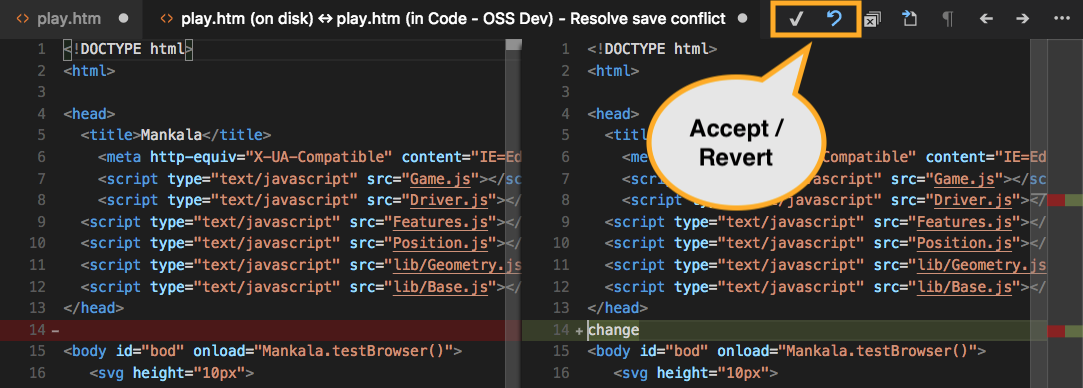
\includegraphics[scale=0.3]{assets/visualstudiocode-merging.png}
		
	\end{center}
	\begin{itemize}
		\item Hint: Use IDEs for Merging: Visual Studio Code! \\
		Source: \url{https://code.visualstudio.com/docs/getstarted/tips-and-tricks#_resolve-merge-conflicts}
		
	\end{itemize}
\end{frame}


\begin{frame}
\frametitle{Thank you}

\begin{center}
	
\includegraphics[scale=0.45]{assets/Change-management-humor.png}
\end{center}

\end{frame}

\begin{frame}
\frametitle{Acknowledgements}

Original version of the Git Vorkurs was kindly provided by 
Lukas Zimmermann. \\

Thanks to all constributors:
\begin{itemize}
\item Lukas Zimmermann
\item Oliver Alka 
\item Simone Lederer
\item Pascal Escher
\end{itemize}


\end{frame}

\end{document}

